\subsection{Актуальность темы}

Во многих задачах анализа данных исходные сведения задаются не точками, а диапазонами. Левая и правая границы интервала могут отражать разброс измерения, неопределённость эксперта или неполноту наблюдения. При этом одинаковое отношение ко всем значениям внутри диапазона часто оказывается слишком грубым. Нечёткая величина позволяет присвоить каждому значению степень принадлежности от 0 до 1 и тем самым сохранить информацию о постепенном переходе от маловероятных к предпочтительным значениям.

Практическая ценность такого представления проявляется в задачах, где требуется сопоставлять неопределённые объекты, выполнять арифметические преобразования и выделять компактные группы. В рассматриваемом проекте нечёткая величина строится из параметров равномерного закона U(a,b). На выбранном уровне α она преобразуется в интервал [A,B], после чего интервалы можно сравнивать, отбирать и кластеризовать. Такое преобразование связывает аппарат нечётких множеств с классическими алгоритмами обработки данных на евклидовой плоскости границ.

Проблема кластеризации в данном случае состоит в том, что объектом анализа является не скаляр, а отрезок. Расстояние должно учитывать обе границы, а центр кластера должен иметь интерпретируемый вид. В библиотеке используется метрика Хаусдорфа для интервалов, которая сводится к максимуму модулей разностей левой и правой границ. Это сохраняет геометрический смысл расстояния и позволяет применять адаптированные варианты k-means++ и пороговой кластеризации.

Отдельную вычислительную проблему создаёт необходимость воспроизводимой генерации наборов. Библиотека не использует внешние генераторы случайных величин. В \texttt{fuzzy/src/rng.cpp} реализованы xoshiro256** и инициализация состояния через splitmix64. Один и тот же seed формирует один и тот же поток псевдослучайных чисел, что необходимо для воспроизводимого эксперимента и сравнения алгоритмов.

\subsection{Объект, предмет и исходные данные проекта}

Объектом исследования является программная система для работы с наборами нечётких величин вида U(a,b) и их α-срезами. Предмет исследования составляют алгоритмы представления, генерации, арифметического преобразования, отбора и кластеризации интервалов.

Исходный код проекта разделён на следующие части:

\begin{itemize}
\item математическое ядро в каталоге \texttt{fuzzy/}, включающее C++17-реализацию типов \texttt{fz\_number}, \texttt{fz\_set}, \texttt{fz\_rng}, арифметики, отбора и кластеризации;
\end{itemize}

\begin{itemize}
\item C API в файле \texttt{fuzzy/include/fuzzy.h}, через который ядро вызывается из внешних языков;
\end{itemize}

\begin{itemize}
\item Go-сервер в каталоге \texttt{server/}, хранящий состояние набора, проверяющий HTTP-запросы и преобразующий данные между JSON, Go-структурами и C API;
\end{itemize}

\begin{itemize}
\item веб-интерфейс \texttt{server/web/}, встроенный в исполняемый файл Go посредством \texttt{go:embed};
\end{itemize}

\begin{itemize}
\item десктопная оболочка \texttt{desktop/}, запускающая локальный сервер и отображающая тот же интерфейс через CEF.
\end{itemize}

Документация \texttt{docs/theory.md} и \texttt{docs/library\_api.md} фиксирует математические определения и контракт внешнего интерфейса. Тестовый набор \texttt{fuzzy/tests/test\_main.cpp} содержит проверки α-срезов, арифметики, генератора, отбора и кластеризации.

\subsection{Цель и задачи курсового проекта}

Цель проекта состоит в разработке и исследовании программного комплекса, который воспроизводимо генерирует нечёткие величины U(a,b), вычисляет их α-срезы и выполняет кластеризацию полученных интервалов с единым C API для C++, Go и других языков.

Для достижения цели решены следующие задачи:

\begin{enumerate}
\item Формализована нечёткая величина в виде функции принадлежности и набора вложенных α-срезов.
\item Реализованы параметрическое представление U(a,b) и дискретное представление произвольной величины через массивы левых и правых границ.
\item Реализованы сложение, вычитание, умножение и деление по интервальной арифметике на каждом уровне α.
\item Реализованы центр тяжести и сравнение по степени возможности.
\item Реализованы xoshiro256**, splitmix64 и генерация наборов с контролируемыми диапазонами начальной точки и ширины.
\item Реализованы отбор по ширине α-среза и по заданному окну.
\item Реализованы k-means++ с заданным числом кластеров и пороговая кластеризация с автоматически определяемым числом кластеров.
\item Создан Go-слой с cgo, HTTP API, импортом и экспортом CSV, журналом и синхронизацией состояния.
\item Проведены модульная верификация и контрольные измерения времени исполнения.
\end{enumerate}

\subsection{Границы применимости}

Библиотека принимает конечные вещественные параметры и проверяет условие \texttt{a < b}. Число уровней задаётся в диапазоне от 2 до 10001, а число генерируемых элементов ограничено диапазоном от 1 до 100000. В Go-сервере выбран фиксированный размер сетки из 21 уровня. Этот режим соответствует интерфейсному сценарию и уменьшает объём передаваемых данных.

Рассматриваемая форма функции принадлежности является монотонно возрастающим треугольником на [a,b]. Для результатов арифметических операций библиотека хранит общую нечёткую величину как вложенные интервалы. Деление запрещается, если носитель делителя содержит ноль. Кластеризация работает с α-срезами одного выбранного уровня, поэтому она не заменяет многомасштабный анализ по нескольким α, а предоставляет анализ фиксированного уровня неопределённости.

Алгоритмы рассчитаны на работу в памяти процесса. Сервер хранит одно текущее состояние набора, защищённое \texttt{sync.Mutex}. Персистентное хранилище, распределённая обработка и межпроцессная база данных в проект не входят.

\begin{figure}[htbp]\centering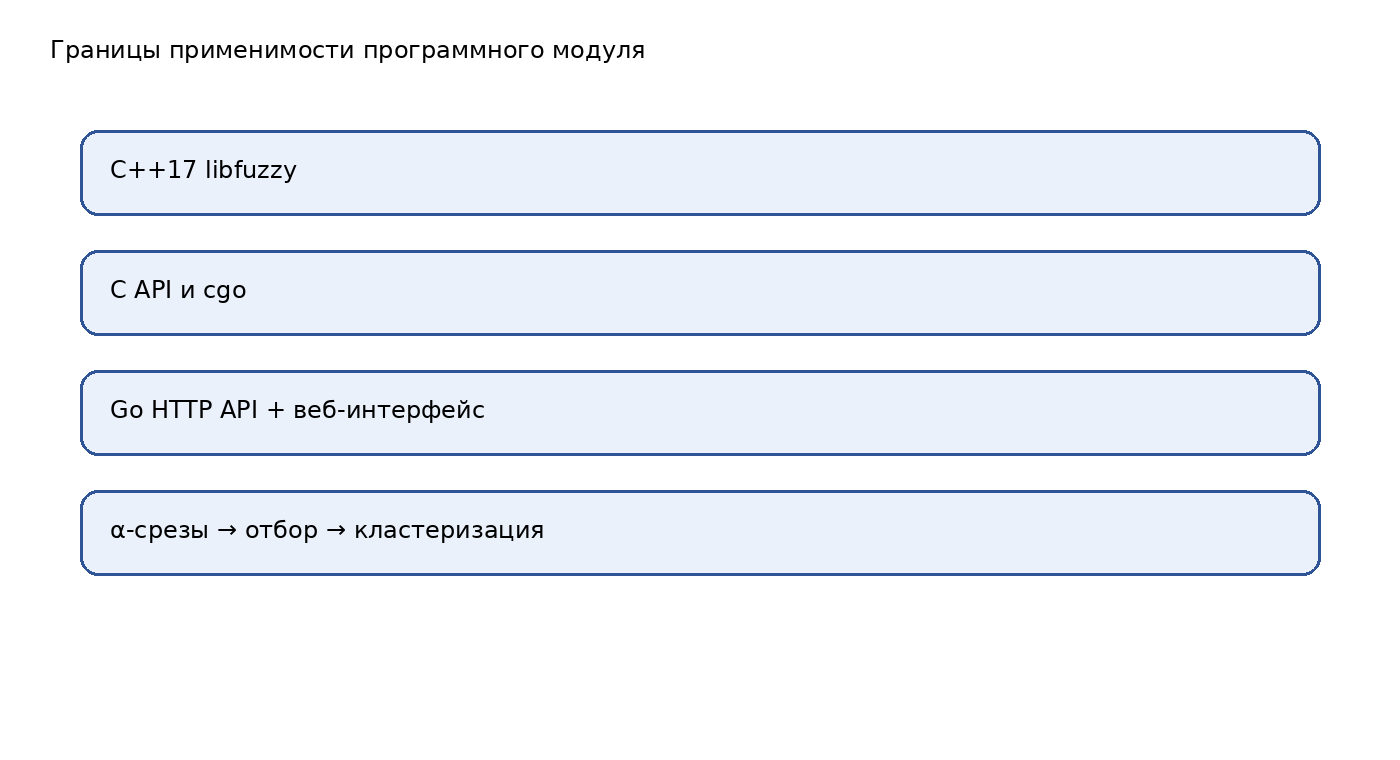
\includegraphics[width=0.9\textwidth]{figures/fig1_scope.png}\caption{схема границ применимости программного модуля}\label{fig:1}\end{figure}

---